% arara: pdflatex 

\documentclass[tikz,border=0pt]{standalone}
\usepackage{pgfplots}
\usepackage{xcolor}
\usepackage{siunitx}

\usetikzlibrary{arrows}

% original colors
\definecolor{color1}{RGB}{166,118,29}
\definecolor{color2}{RGB}{217,95,2}
\definecolor{color3}{RGB}{231,41,138}
\definecolor{color4}{RGB}{117,112,179}
\definecolor{color5}{RGB}{27,158,119}
\definecolor{color6}{RGB}{102,166,30}
\definecolor{color7}{RGB}{230,171,2}

\definecolor{amber(sae/ece)}{rgb}{1.0, 0.49, 0.0}

\def \imscale {0.31}

\begin{document}
\begin{tikzpicture}
\clip (-5.59cm, -3.6cm) rectangle (5.59cm, 3.49cm);

\node[inner sep=0pt] (image) at (0,0)
{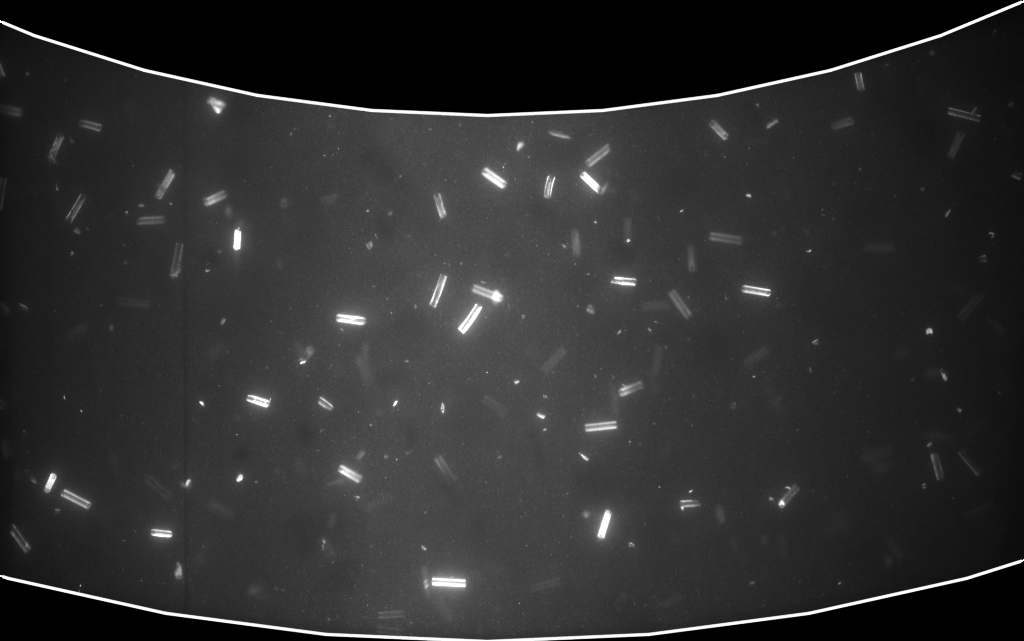
\includegraphics[scale=\imscale]{stillimage.png}};

\draw[color=amber(sae/ece), line width=0.7mm] (-0.28, 16.75) circle (14.5);
\draw[color=amber(sae/ece), line width=0.7mm] (-0.28, 16.75) circle (20.24);

% scale bar

\begin{scope}[
    xshift=4.2cm,
    yshift=-2.1cm,
]
   \fill[fill=white, fill opacity=0.25] (-3.5mm, -0.50mm) rectangle (7.0mm, 6.0mm);

   \draw [white, line width=0.25em] (0,1.2em) --
       node[below,inner sep=0.1em, font=\large] {\SI{5}{\milli\meter}}
       %(1 / \imscale * 5mm * 33 / 80mm, 1.2em);
       (3.5mm, 1.2em);
\end{scope}

\begin{scope}[
    xshift=-0.3cm,
    yshift=2.9cm,
    ->,
    >=stealth',
    very thick,
]
  \node at (-3cm,0) (1) {};
  \node at (3cm,0) (2) {};
  %\path[white] (2) edge[bend left=10] node [above] {\huge$\omega_i$} (1);
  \path[white] (2) edge[bend left=10] node [above] {\Large Inner cylinder} (1);

\end{scope}

\end{tikzpicture} 
\end{document}
